%\section{Related Work}\label{Related}


\section{尺度不變特徵向量(Scale Invariant Feature Transform)}
%SIFT 特徵點描述方法
	尺度不變特徵向量(SIFT) 一開始由 lowe \cite{Lowe2004} 所提出,目的是尋找兩張圖片中的相似特徵向量來比對兩張圖片的相對關係,主要分成四個階段:
\begin{itemize}
	\item (1) 區域空間極值分布
    \item (2) 特徵點定位與篩選
    \item (3) 特徵點方向分配
    \item (4) 特徵點描述向量建立
\end{itemize}

   第一階段(1) 區域空間極值篩選,先利用不同尺度間的高斯金字塔選擇區域中的最大極值,其高斯分布式子如下:
\begin{align}
  G(x,y,\sigma) = \frac{1}{2\pi\sigma^2}exp(-(x^2+y^2)/2\sigma^2) 
\end{align}

	不同尺度的高斯分布利用摺積 (Convolution) 將影像模糊化。 $I(x,y)$代表原始影像,$G(x,y,\sigma)$代表高斯函數:
	
\begin{align}
  L(x,y,\sigma) = G(x,y,\sigma)\ast{I(x,y)}
\end{align}

    再利用每組影像相鄰的高絲模糊影像進行高斯差分(Difference-Of-Gaussian),目的用於在集合內4組高斯差分影像中找出極值,式子如(1.3)所示:
    
\begin{align}
  D(x,y,\sigma) = L(x,y,k\sigma)-L(x,y,\sigma)
\end{align}

  在此k為高斯模糊的尺度比值,設為$\sqrt{2}$,若某個像素的極值為26個相鄰的像素中最大或最小的話,則此像素的位址即為區域極值的所在。

  第二階段(2) 特徵點定位篩選,其主要的目的在於找出真正有用的特徵點,在此特徵點的精準度必須要達到次像素的精度。有的特徵點其極值為低對比度的點,這時候這些低對比度的特徵點就會不予採用,剩下的特徵點即可為
下一階段所使用。作法首先將(1.3)利用泰勒展開得到(1.4):
 
\begin{align}
  D(x) = D + \frac{\delta D^T}{\delta X}X + \frac{1}{2}X^T\frac{\delta^2 D}{\delta X^2}X
\end{align}

   式中$X$為極值$(x,y,\delta)^T$,$D$為高斯差分後的結果,再將(1.4)對$X$作偏微分可得$\vec{X}$算出$X$為極值點的的偏移量。
   
\begin{align}
  \vec{X} = -\frac{\delta^2 D}{\delta X^2}^{-1}\frac{\delta D}{\delta X}
\end{align}   
   
   
   若是$\vec{X} >= 0.5$,或是 $\sigma > k/2$,表示此區域極值點較靠近相鄰的點位,則需要再將此點移至相鄰的極值再經(1.5)計算後得到最佳的位置。若將$\vec{X}$帶入(1.4)中,可得(1.6)我們所用來篩選的式子:
   
\begin{align}
  D(\vec{X}) = D+\frac{1}{2} \frac{\sigma D^T}{\sigma X} \vec{X}
\end{align}      
   
   利用(1.6)將求出的絕對值與其他絕對值相比,可將對比度小的特徵點刪除以達到過濾的效果。
   
   第三階段(3) 特徵點方向分配,目的在於當對比的圖片有旋轉或者是尺度上的變化,相同的特徵點為了保有相同方向的特性,必須賦予每個特徵點一組特定的方向。其做法則是利用統計的方式,將所有的梯度值以角度每10個單位做方位直方圖記錄,
並且記錄每個梯度的強度,以(1.7)(1.8)表示:

\begin{align}
	\theta (x,y)= tan^{-1}(\frac{\delta L}{\delta y}/\frac{\delta L}{\delta x}))
\end{align}      
   
\begin{align}
	m(x,y) = \sqrt{(\frac{\delta L}{\delta x})^2+(\frac{\delta L}{\delta y})^2}
\end{align}



\begin{figure}[htbp] %
\centering 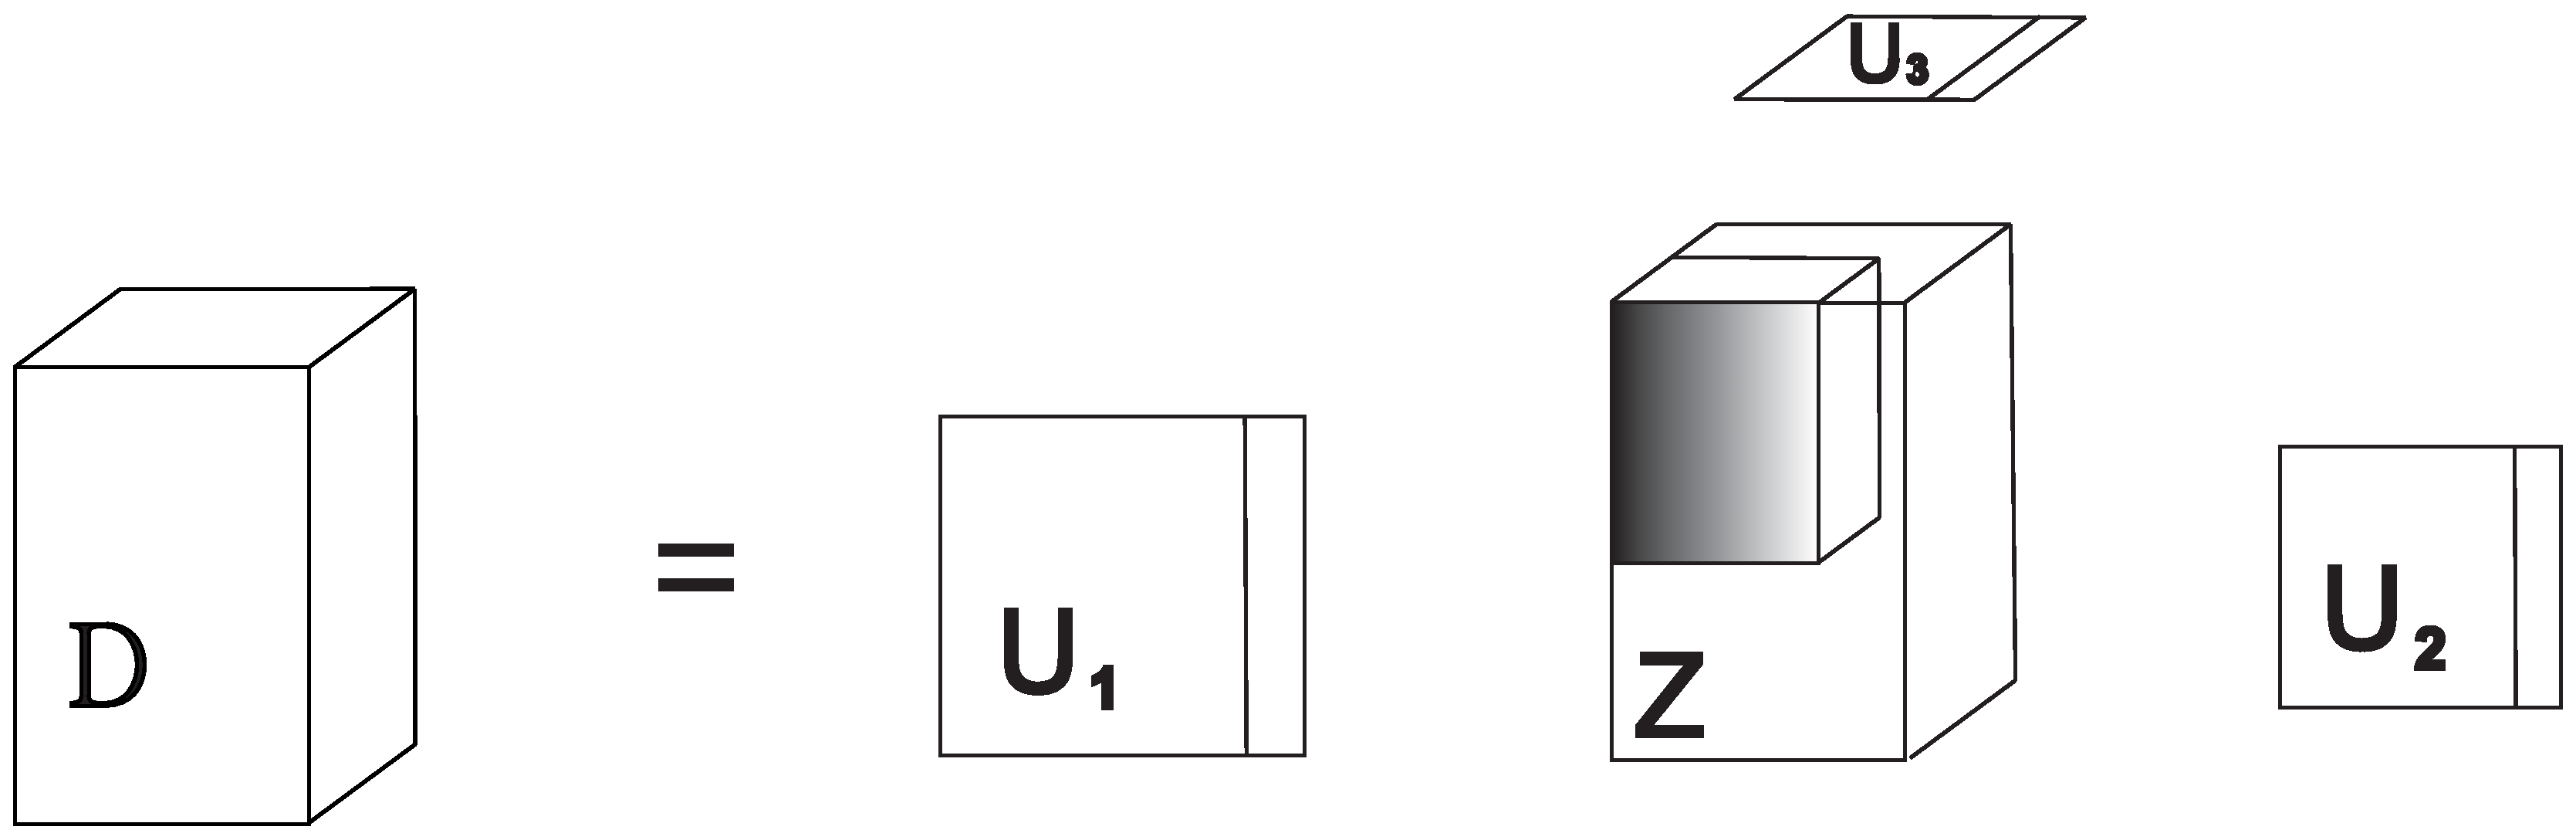
\includegraphics[width=8cm,keepaspectratio
  ]{figures/coretensor.eps}
\caption{An $N$-mode SVD orthogonalizes the $N$ vector spaces associated with an order-$N$ order (the case $N=3$).}
\label{fig:N-mode}
\end{figure}